% Roll Number 1, Aadil Abdul Latheef K P

\textbf{\textcolor{LightMagenta}{Define VC dimension. Show that VC dimension of a line hypothesis is three. (Dec 2019) \hfill 4 marks}} \\[5pt]
The \textbf{Vapnik-Chervonenkis dimension}, VC(H), of hypothesis space H defined over instance space X is the size of the largest finite subset of X shattered by H. If arbitrarily large finite sets of X can be shattered by H , then \[VC(H)\equiv\infty.\]
For a given decision function (classification function), the VC dimension indicates the maximum number of training sets that can be classified without any error. If there are three points in the same two-dimensional space, it can be shattered with line function machine into eight $(2^3)$ combination without error during training in the following manner.\\
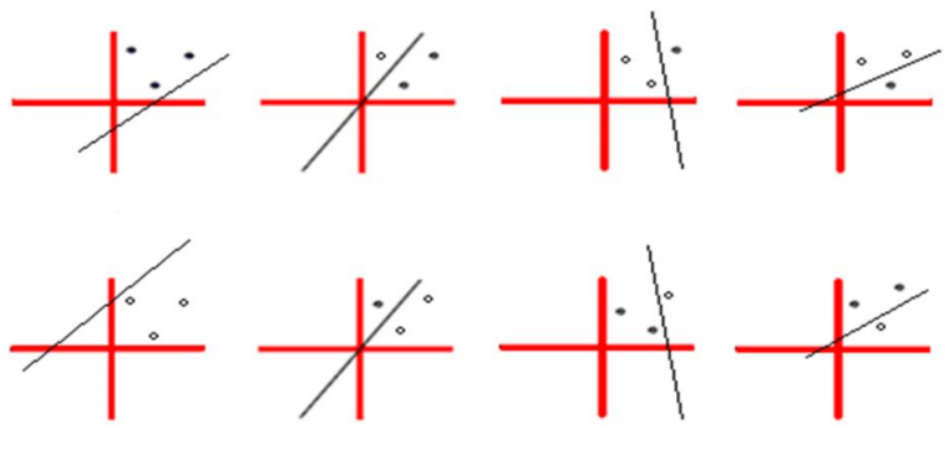
\includegraphics[scale=0.5]{Images/A35_img1.png}\\
In a two dimensional space, the maximum number of training points that can be shattered by the line function is 3.Hence for line function VC dimension h=3.